\chapter{Temperature and Emissivity Separation}
\label{chap:TES}

Many applications of airborne thermal hyperspectral data are based on derivation of temperature and emissivity from the pre-processed image. These quantities are obtained from the system of RTEs. Let us remind that every spectral band follows RTE as shown in \ref{eq:RTE}. Thus, in the case of TASI sensor one obtains system of 32 RTEs. Atmospheric transmittance $\tau$, atmospheric upwelling radiance $L_\mathrm{atm}^\uparrow$ and atmospheric downwelling radiance $L_\mathrm{atm}^\downarrow$ are determined during atmospheric corrections as discussed in the Chapter \ref{chap:Data}. Note that even after the compensation of the atmosphere, the system of RTEs in case of TASI sensor contains 32 unknown emissivities and also unknown temperature, which is the same in all spectral bands. It results in the underdetermined system of equations. The estimation of temperature and emissivity from such a system of equations is usually addressed as temperature-emissivity separation. This chapter describes several approaches for separating temperature and emissivity. It firstly introduces few commonly used ones and then focuses on the most popular approach called \textit{Temperature and emissivity separation algorithm}. Finally it discusses its possible improvement together with its validation.

\section{Available approaches}

Algorithms used for processing airborne thermal hyperspectral data are mostly focused on atmospheric correction and on estimation of temperature and emissivity. Procedures and algorithms for atmospheric correction will be mentioned just briefly. The attention will be focused on algorithms used for estimation of temperature and emissivity since this topic is further investigated as reported in section four.

Methods used to overcome the problem of underdetermined system of RTEs are usually based on adding empirical or semiempricial constraints. Review written by Li et al. \cite{LZ13} sums up currently used methods for spaceborne sensors. Just a few of the methods can be applied for processing of data from airborne sensors. The main reason is that satellites acquires images periodically and algorithms takes advantage of it. This requirement is difficult to fulfill with thermal airborne sensors. In following are mentioned four algorithms, which are commonly used in processing of airborne thermal hyperspectral data.

\subsubsection*{Gray body emissivity method}

Barducci and Pippi \cite{BP96} proposed algorithm, which is based on assumption of flat spectral emissivity beyond $\SI{10}{\micro\meter}$. To solve the system of RTEs it is enough to find at least two spectral bands with the same emissivity. This can be achieved in case of airborne thermal hyperspectral data. Drawback of this method is its sensitivity to instrument noise.

\subsubsection*{Linear emissivity constraint temperature emissivity separation method}

As Wang et al. \cite{WW11} describe, this method is based on idea of substituting spectral emissivity with piecewise linear function. The emissivity spectrum is divided into segments, in which spectral emissivities are assumed to be linearly dependent on wavelength. Thus, it is necessary for every segment to estimate gain and offset. It implies that the number of spectral bands has to be equal or greater than number of unknowns resulting from segmentation to piecewise linear functions.

\subsubsection*{Spectral smoothing}

Spectral smoothing algorithm, also known as ARTEMISS (Automatic Retrieval of Temperature and EMIssivity using Spectral Smoothness), was reported by Borel at \cite{B98} and \cite{B07}. Algorithm is based on the assumption that spectra of solids are much more smoother than spectra of gases. Thus by smoothing spectra one removes spectral features introduced by atmosphere and obtains spectral emissivity. Moreover, current implementation described in \cite{B07} includes modified ISAC algorithm called ARTISAC, which estimates atmospheric transmissivity for further choice correct atmospheric model. Atmospheric models contains so called TUD (atmospheric Transmissivity, Upwelling and Downwelling atmospheric radiance) and are stored in look-up tables (LUT). Then temperature is varied until the spectral emissivity is the smoothest possible, where the smoothness criterion is standard deviation of measured radiance minus simulated radiance. Spectral smoothness method can be described briefly by following steps:
\begin{enumerate}
	\item estimation atmospheric transmissivity using ARTISAC algorithm
	\item determination few closest atmosphere models from TUD-LUT according to the estimated atmospheric transmissivity
	\item use these atmosphere models as input to spectral smoothness algorithm for a few pixels chosen from the image and the atmosphere model which results in smoothest emissivity in the most of the cases is chosen as the correct one
	\item use chosen atmosphere model for the whole image and estimate temperature and emissivity using spectral smoothness
\end{enumerate}

\subsubsection*{Temperature and emissivity separation algorithm}

Temperature and emissivity separation algorithm was originally developed for Advanced Spaceborne Thermal Emission and Reflection Radiometer (ASTER) sensor on board Terra platform. The algorithm is summarized by Gillespie et al. \cite{GR98} and is described in detail in \cite{G99}. It relies on the semi-empirical relationship between the spectral contrast and the minimum spectral emissivity. The algorithm consists of three modules, namely Normalization Emissivity Module (NEM) reported by Gillespie \cite{G95}, ratio module and Maximum-Minimum Difference (MMD) module reported by Matsunaga \cite{M94}. The inputs of the algorithm are land-leaving radiance $L_{LL}$ and downwelling radiance $L^{\downarrow}_{atm}$. Land-leaving radiance can be obtained from RTE by compensating for atmospheric transmissivity $\tau$ and atmospheric upwelling radiance $L^{\uparrow}_{atm}$:
$$ L_{LL} = \varepsilon B(T_s) + (1 - \varepsilon) L^\downarrow_{atm}. $$

The NEM module consists of iterative process of estimating temperature and emissivity, and compensating for the downwelling radiance. The output of the NEM module is initial temperature and emissivity estimation. Then ratio module performs ratioing of the emissivities obtained by NEM module to its arithmetic mean. Thus one obtains so called $\beta$ spectrum which should be less sensitive for sensor noise. Finally, maximum and minimum of $\beta$ spectrum is found and its difference (MMD) is used in following relationship:
\begin{equation} \varepsilon_{min} = 0.994 - 0.687 \times \text{MMD}^{0.737}. \label{eq:MMD} \end{equation}
Derivation of equation \ref{eq:MMD} is explained in following paragraph. Ratioing $\beta$ spectrum back to emissivity spectrum with knowledge of minimum emissivity results in more precise emissivity estimation. The band with highest emissivity is used for temperature estimation. Such an estimation of temperature and emissivity is passed through the ratio and MMD module once again and those results are considered to be final.

The relationship between emissivity contrast and minimum spectral emissivity is regression based on 86 laboratory spectra of rocks, soils, vegetation, snow and water chosen from ASTER spectral library \cite{BH09}. This relationship is shown in figure \ref{fig:EpsMinMMD}. It is important to emphasize that equation \ref{eq:MMD} is tailored for ASTER sensor. Nevertheless the algorithm can be applied for airborne sensors as well performing small modification. To apply temperature and emissivity separation algorithm to different sensor, regression of $\varepsilon_{min}$ on MMD needs to be refined using sensor specific response functions. Temperature and emissivity separation algorithm was applied for example to AHS sensor as reported in \cite{SJ06} or to TASI sensor as reported in \cite{PP12} or \cite{WQ11}.
\begin{figure}[htb]
	\centering
	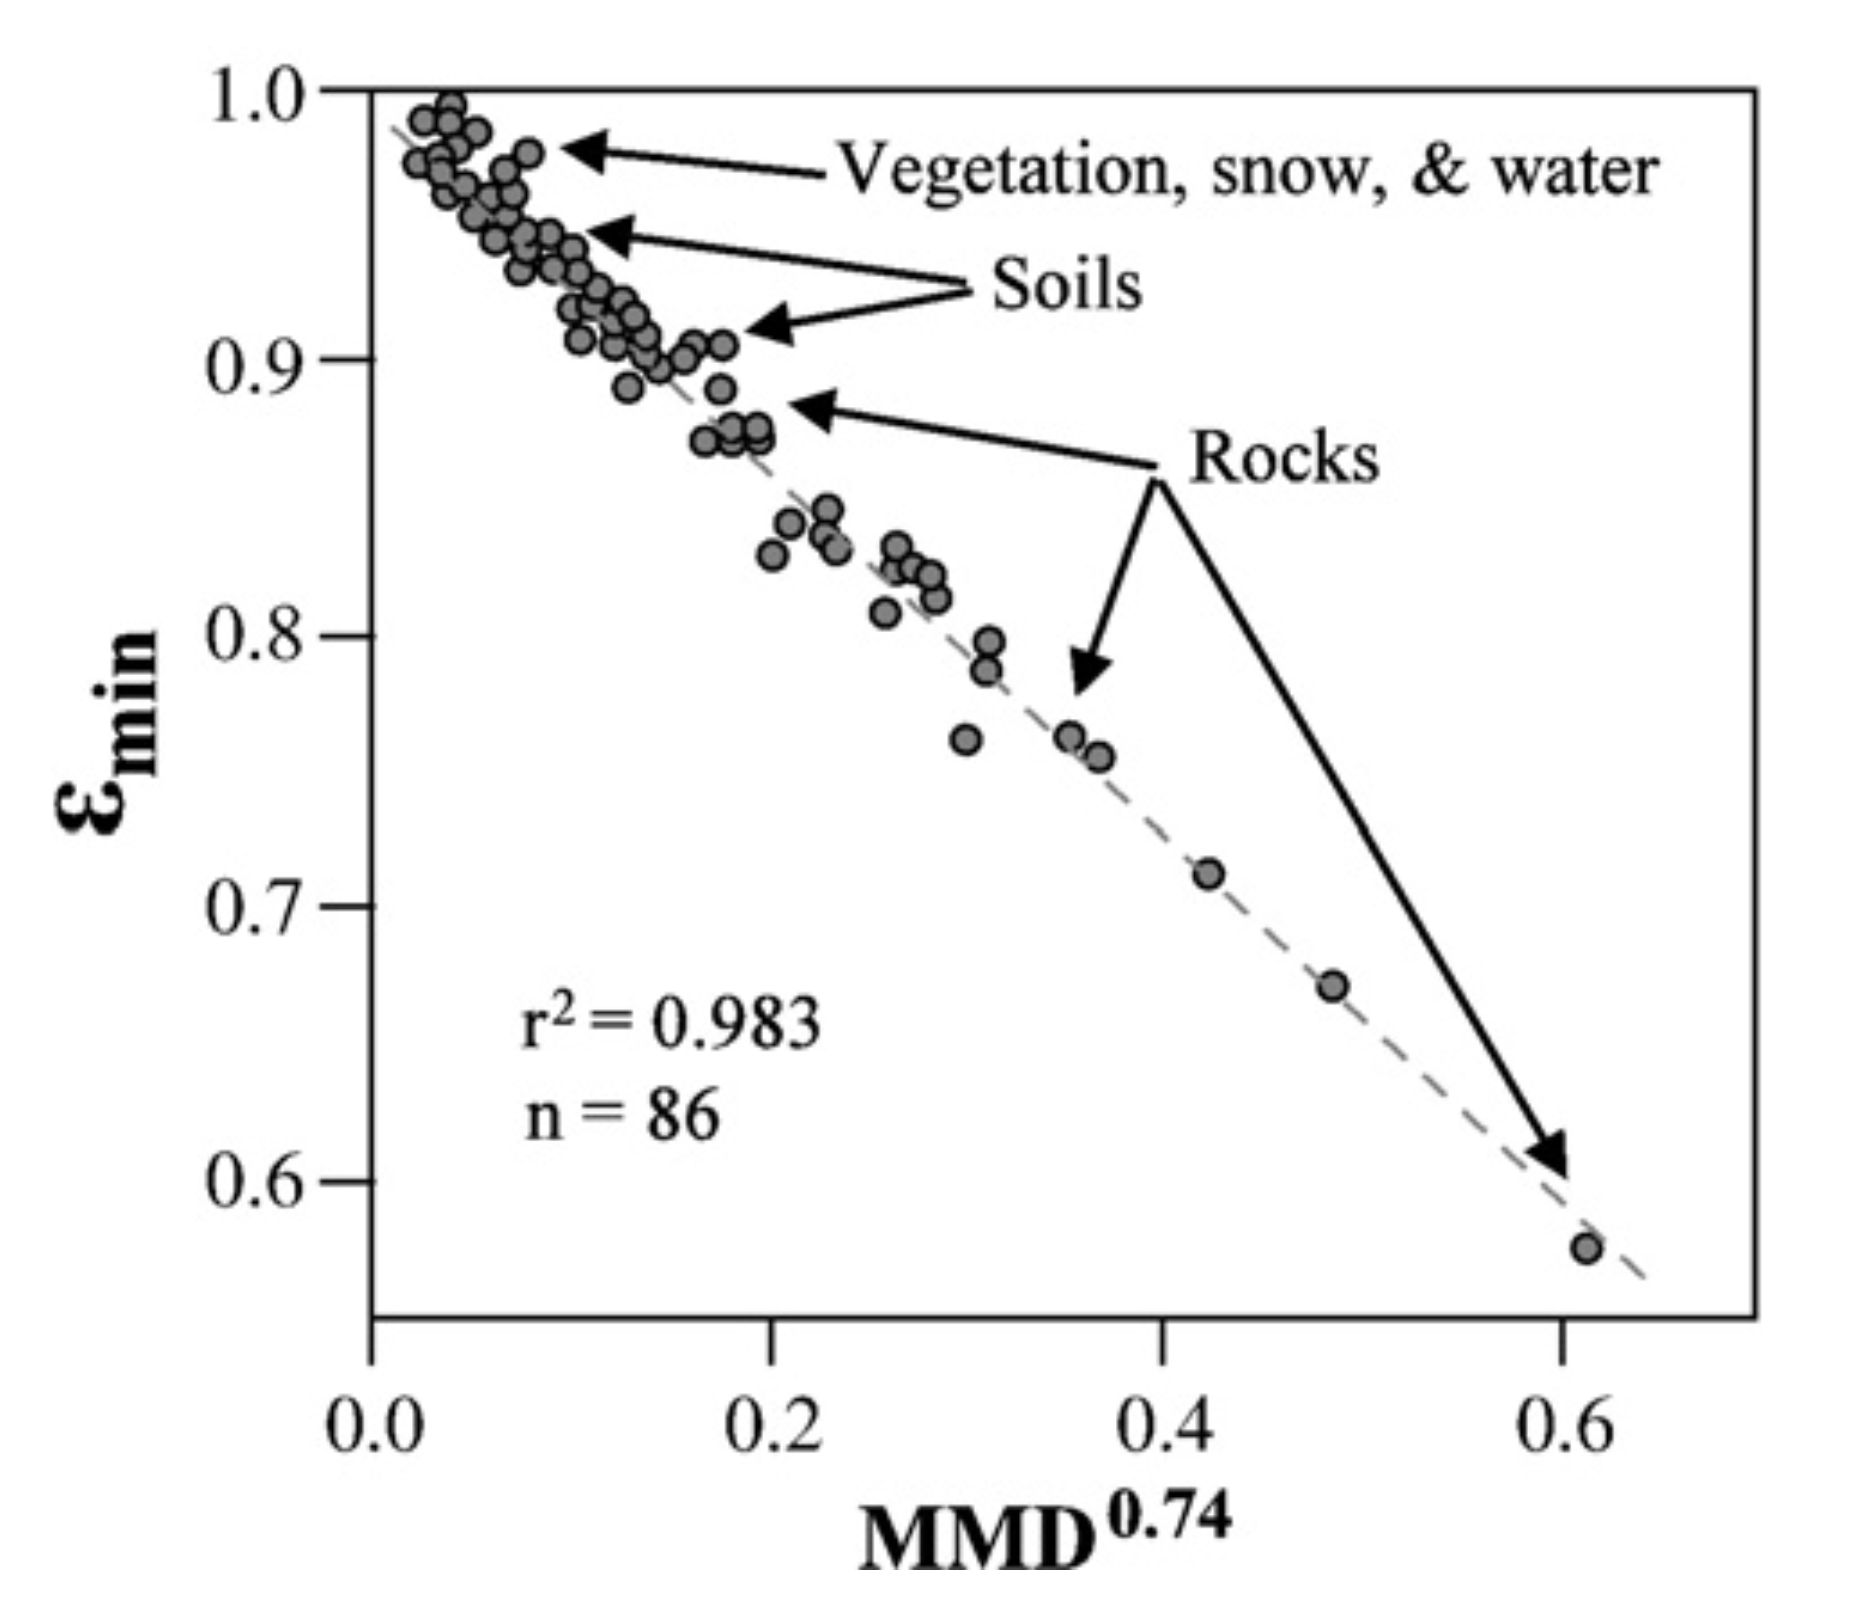
\includegraphics[scale=0.2]{pics/Chapter_03/EpsMinMMD.png}
	\caption{Semi-empirical relationship between emissivity contrast and minimum spectral emissivity as shown in study reported by Sabol et al. \cite{SG09}.}
	\label{fig:EpsMinMMD}
\end{figure}

Samples with small spectral emissivity contrast are treated as gray body with constant emissivity $\varepsilon=0.985$. These samples are detected mainly by comparing its spectral contrast with predefined MMD threshold. The MMD threshold for low-contrast samples, equation \ref{eq:MMD} and number of iteration in NEM module slightly differ with different versions of temperature and emissivity separation algorithm as reported by Sabol et al. \cite{SG09}.

\section{TES Algorithm Improvement}

The algorithm described below brings a new approach for the TES algorithm by replacing the NEM module with a completely new module. The main idea of the new module is based on the relationship  between brightness temperature $T_\mathrm{b}$ and emissivity, where brightness temperature is the temperature obtained from land-leaving radiance under assumption of emissivity $\varepsilon=1$. The algorithm description below omits all wavelength notation for clarity reasons. In order to demonstrate the relationship, three emissivity samples with different spectral contrasts were chosen from the ASTER spectral library \cite{baldridge_aster_2009}. These emissivities were applied to Plank's law at temperature $300\,\mathrm{K}$. The resulting radiance, as well as the emissivity samples, were transformed to band-effective quantities with repsect to the ASTER, AHS and TASI response functions. Brightness temperatures for every band of each sensor were obtained by appling inverse Planck's law on sample radiance under the assumption of unit emissivity. The results, shown in Fig. \ref{fig:relationship}, clearly exhibit the relationship between emissivity and brightness temperature with linear trend, no matter what spectral contrast is or what type of sensor is used.

\begin{figure}[htb]
	\centering
	\vspace{1em}
	\begin{subfigure}[t]{.3\linewidth}
		\centering
		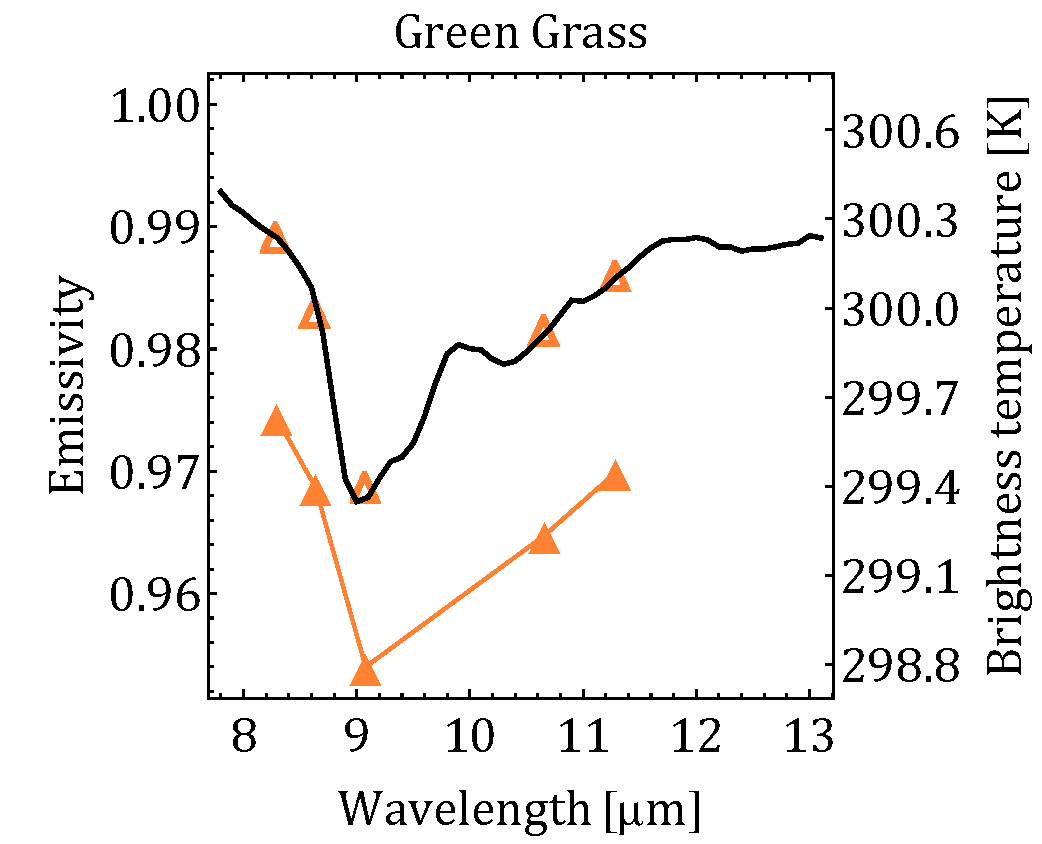
\includegraphics[scale=0.3]{pics/Chapter_03/pivov2.pdf}
		\vspace{-0.1cm}
		\caption{}
		\label{fig:BBradiation}
	\end{subfigure}
	\hspace{1em}
	\begin{subfigure}[t]{.3\linewidth}
		\centering
		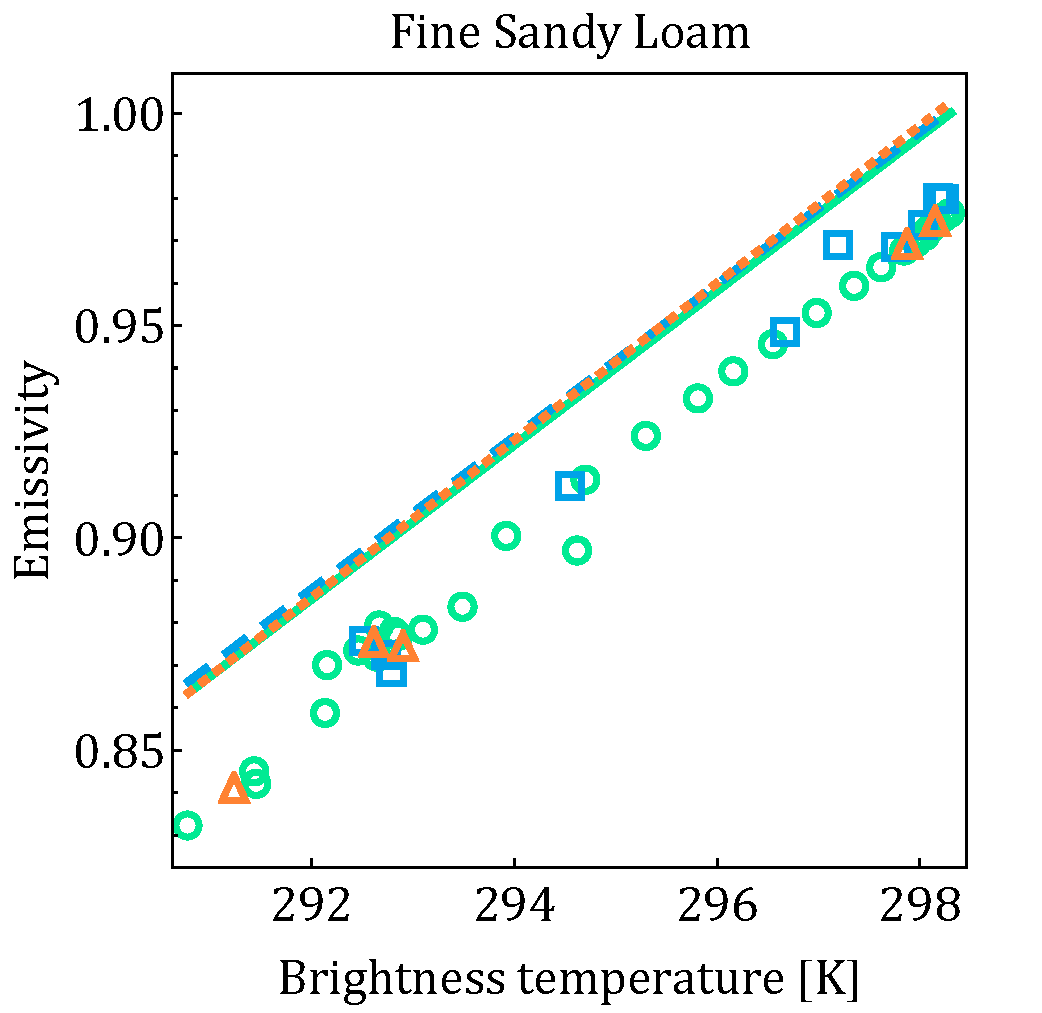
\includegraphics[scale=0.3]{pics/Chapter_03/pivov3.pdf}
		\vspace{-0.1cm}
		\caption{}
		\label{fig:QuartzEmissivity}
	\end{subfigure}
	\hspace{1em}
	\begin{subfigure}[t]{.3\linewidth}
		\centering
		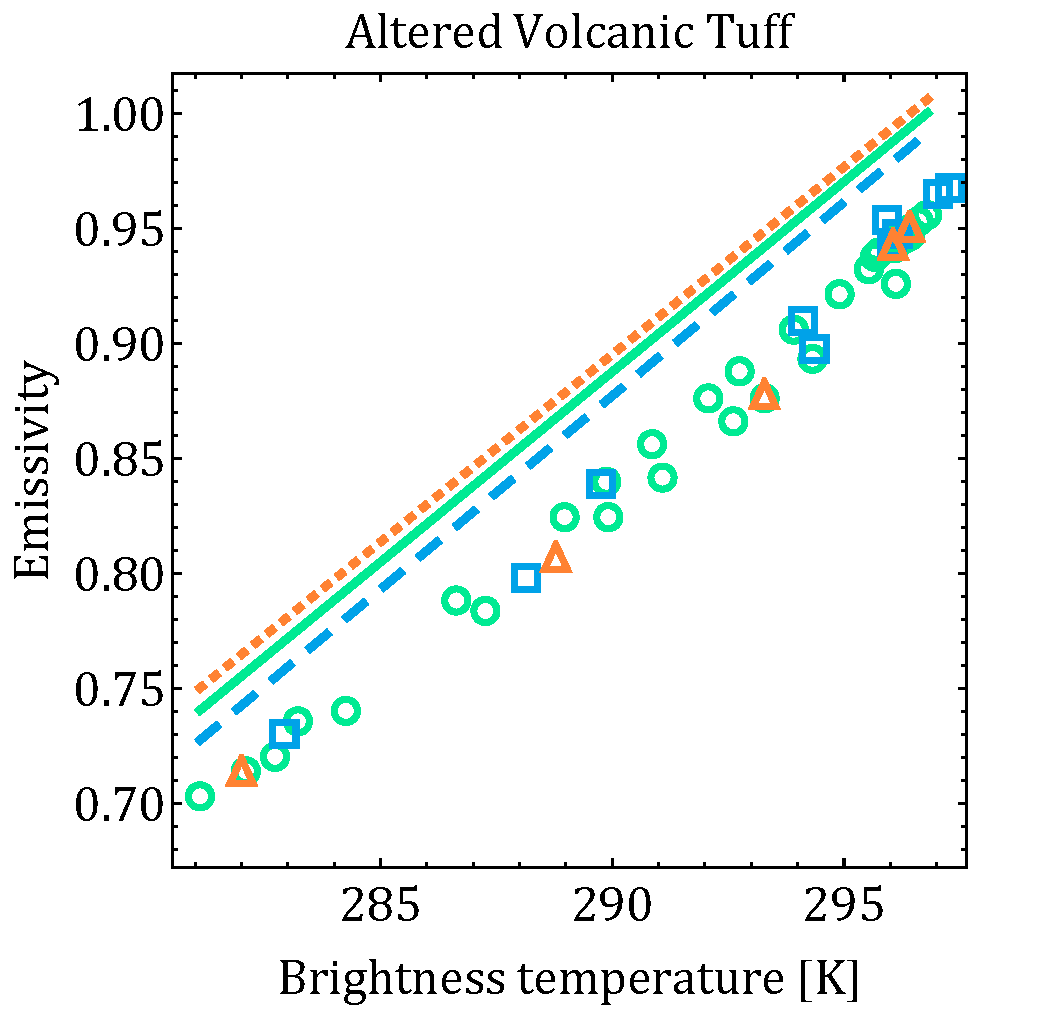
\includegraphics[scale=0.3]{pics/Chapter_03/pivov4.pdf}
		\vspace{-0.1cm}
		\caption{}
		\label{fig:QuartzRadiance}
	\end{subfigure}
	\vspace{1.5 em}
	\caption{Symbols represents examples of the relationship between brightness temperature $T_\mathrm{b}$ and emissivity as would be observed by ASTER (orange triangles), AHS (blue squares), and TASI (green circles). Lines illustrate the approximations of the relationship between brightness temperature and emissivity for ASTER (orange dotted line), AHS (blue dashed line), and TASI (green full line) sensor. The procedure used for estimation the brightness temperature and emissivity relationship is described in text.}
	\label{fig:relationship}
\end{figure}

This property will be further used for emissivity estimation. The dependence of emissivity on brightness temperature will be approximated by following equation:
\begin{equation} \varepsilon = a T_\mathrm{b} + b, \label{eq:relationship}\end{equation}
where $a$ and $b$ are empirical coefficients. These coefficients are determined by solving the system of two equations using two points, namely maximum brightness temperature coupled with emissivity equal to 1 and minimum brightness temperature coupled with lowest emissivity $\varepsilon_\mathrm{min}$:
\begin{equation}
\begin{aligned}
	1 &= a \max (T_\mathrm{b}) + b, \\
	\varepsilon_\mathrm{min} &= a \min (T_\mathrm{b}) + b.
\end{aligned}
\label{eq:sytemofeq}
\end{equation}
The next step is estimation of the the lowest emissivity $\varepsilon_\mathrm{min}$.

This is done by varying $\varepsilon_\mathrm{min}$ over the range $[0.4,1)$, determining corresponding coefficients $a$ and $b$ by solving (\ref{eq:sytemofeq}) and then approximating emissivity by (\ref{eq:relationship}) using brightness temperature for all spectral bands. The estimated emissivity is then used together with land-leaving radiance $L_\mathrm{LL}$ and downwelling radiance $L^\downarrow$ in a computation that yields spectral radiance:
\begin{equation}
	L^{\prime} = \frac{L_\mathrm{LL}-(1-\varepsilon)L^\downarrow}{\varepsilon}.
\end{equation}
The temperature in every spectral band is derived from spectral radiance $L^{\prime}$ applying inverse Plank's law. The highest one is chosen as the reference temperature $T_\mathrm{max}$. Finally, the estimated spectral radiance $L^{\prime}$ and Planck's law at the reference temperature $T_\mathrm{max}$ are normalized and compared against each other as follows:
\begin{equation}
	\sum_{\lambda_i} \left| \frac{B(T_\mathrm{max})}{||B(T_\mathrm{max})||_1} - \frac{L^\prime}{||L^\prime||_1} \right|,
\end{equation}
where $\lambda_i$ is the $i-$th band effective wavelength. The value of $\varepsilon_\mathrm{min}$ is considered final if its corresponding spectral radiance $L^{\prime}$ fits Planck's law the best.

The whole process of determining $\varepsilon_\mathrm{min}$ can be understood as smoothing the spectrum by finding the optimal value of $\varepsilon_\mathrm{min}$. Pseudocode depicted in Fig. \ref{fig:FunctionCode} summarizes the above described procedure as a function \textsc{SmoothingErr}($\varepsilon_\mathrm{min},L_\mathrm{LL},L^\downarrow$) evaluating the error between Planck's law and estimated spectral radiance. This function is minimized with respect to the variable $\varepsilon_\mathrm{min}$ as follows:
\begin{equation}
\underset{\varepsilon_\mathrm{min} \in [ 0.4 ,1 )}{\text{arg\,min}}\:\text{\textsc{SmoothingErr}}(\varepsilon_\mathrm{min},L_\mathrm{LL},L^\downarrow).
\label{eq:costFunction}
\end{equation}

Continuous curves in Fig. \ref{fig:relationship} show the optimal brightness temperature and emissivity relationship approximation. Let us emphasize that the emissivity approximated by (\ref{eq:relationship}), as a result of the above described procedure, tends to be overestimated, which can be observed in the Fig. \ref{fig:relationship} as well. This behavior causes the temperatures, derived from spectral radiance $L^{\prime}$, to be underestimated. Therefore the maximum temperature is likely to be the closest to the true temperature and is taken as the reference temperature.

Before passing emissivty to the Ratio and MMD modules, it is refined according to (\ref{eq:emissivityComputation}):
\begin{equation}
\varepsilon = \frac{L_\mathrm{LL} - L^\downarrow}{B(T) - L^\downarrow},
\label{eq:emissivityComputation}
\end{equation}
where $T$ is the maximum temperature associated with optimal $\varepsilon_\mathrm{min}$. The emissivity is then further processed with the Ratio and MMD modules, with minor changes to original version of the TES algorithm as it is described in \cite{gillespie_temperature_1998} and \cite{gillespie_temperature/emissivity_1999}. These changes include: 1) there is no refinement of $\varepsilon_\mathrm{max}$ according to the emissivity spectral contrast, 2) the threshold $T_1$ for separation emissivities with small spectral contrast is not applied, and 3) the number of MMD iterations is set to one. Let us emphasize, that before  
reporting algorithm outputs, emissivity is refined by (\ref{eq:emissivityComputation}) using final value of temperature.

\section{Algorithm Performance}

The OSTES algorithm was tested on synthetic data and on data acquired with the ASTER sensor. The results show that the OSTES algorithm improves temperature and emissivity retrievals in several ways. The most significant improvement occurs for surfaces with low spectral contrast, which is one of the major weaknesses of the original version of TES algorithm. The temperature and emissivity estimations from OSTES are more accurate in these cases. The investigation of OSTES with simulated data also shows that the algorithm is less sensitive to seasonal fluctuations in atmospheric and surface temperature.

\section{Simulated Data}

A data set of 6588 samples was artificially created to compare the performance of the TES and OSTES algorithms. Samples include 108 different natural surfaces chosen from ASTER spectral library \cite{baldridge_aster_2009} at different temperatures coupled with 61 different atmospheric conditions taken from TIGR (TOVS Initial Guess Retrieval) database \cite{chedin_improved_1985, chevallier_neural_1998}. 
These samples were processed to land-leaving and downwelling radiance, as standard TES algorithm input, and they were transformed to band-effective quantities with respect to the ASTER, AHS and TASI response functions.

Simulated data for the ASTER sensor were processed with current implementation\footnote{We were unable to obtain the original TES code, so we have implemented it according to the ATBD \cite{gillespie_temperature/emissivity_1999} with revisions as described in \cite{gustafson_revisions_2006} and \cite{sabol_field_2009}. We were, however, successful in getting our simulated data processed with the operational TES code.} of TES, as it is used for generation of ASTER standard products AST\_05 and AST\_08 \cite{bjorn_personal_communication}. The version of the original TES algorithm in cases of AHS and TASI sensors was implemented in a manner similar to that described in \cite{jimenez-munoz_surface_2012}. In addition, the implementation omits the $\varepsilon_\mathrm{max}$ refinement for emissivities with low spectral contrast. The OSTES was applied to all sensors as it is described in previous section.

\begin{table}[!t]
\renewcommand{\arraystretch}{1.5}
\caption{Standard deviations of temperature errors obtained by applying OSTES and TES algorithm on simulated data as seen by ASTER, AHS and TASI grouped according to the sample Maximum-Minimum emissivity Difference (MMD). }
\label{table:StandardDeviations}
\centering
\begin{tabular}{cccc}
\hline
Sensor & MMD & OSTES & TES \\ \hline
ASTER 	& $< 0.021$ & 0.25 & 0.50 \\
 		& $> 0.021$ & 0.36 & 0.43 \\ \hline
AHS 		& $< 0.052$ & 0.13 & 0.20 \\
 		& $> 0.052$ & 0.20 & 0.19 \\ \hline
TASI 	& $< 0.026$ & 0.16 & 0.32 \\
 		& $> 0.026$ & 0.32 & 0.30 \\
\hline
\end{tabular}
\end{table}

Samples were passed to the TES and OSTES algorithms and the temperature and emissivity results were compared with true values. We divide the results into two groups according to the emissivity spectral contrast. For each sensor type we determined a threshold for Maximum-Minimum emissivity Difference (MMD) in order to separate the samples with small spectral contrast such as water, vegetation, snow or samples with small particle sizes from other samples with higher spectral contrast. The threshold was determined for each sensor separately since different response functions and spectral ranges result in different MMD values for the same sample. The performance of both TES versions was determined by subtracting retrieved temperature from true temperature value. The temperature error and chosen MMD values for ASTER, AHS and TASI are shown in Fig. \ref{fig:SimualtedDataTemperatureErrorVsLowVsHighMMD}.

It can be seen that temperature and emissivity retrieved with OSTES are more accurate for samples with low spectral contrast. On the other hand, no significant improvement is evident in cases of samples with higher spectral contrast. 

Let us remind the reader that every sample is processed under several different atmospheric conditions coupled with different sample temperatures. Thus the standard deviation of temperature and emissivity error is indicative of the algorithm’s sensitivity to seasonal fluctuations. A comparison of standard deviations of temperature errors introduced by both TES approaches reveals that the OSTES is less sensitive to changes in atmosphere and sample temperature for samples with low MMD. However, the standard deviations of temperature errors of samples with higher MMD are similar. Standard deviations of temperature errors obtained by the OSTES and TES algorithms are summarized in the Table \ref{table:StandardDeviations}.

\begin{figure*}[!t]
\centering
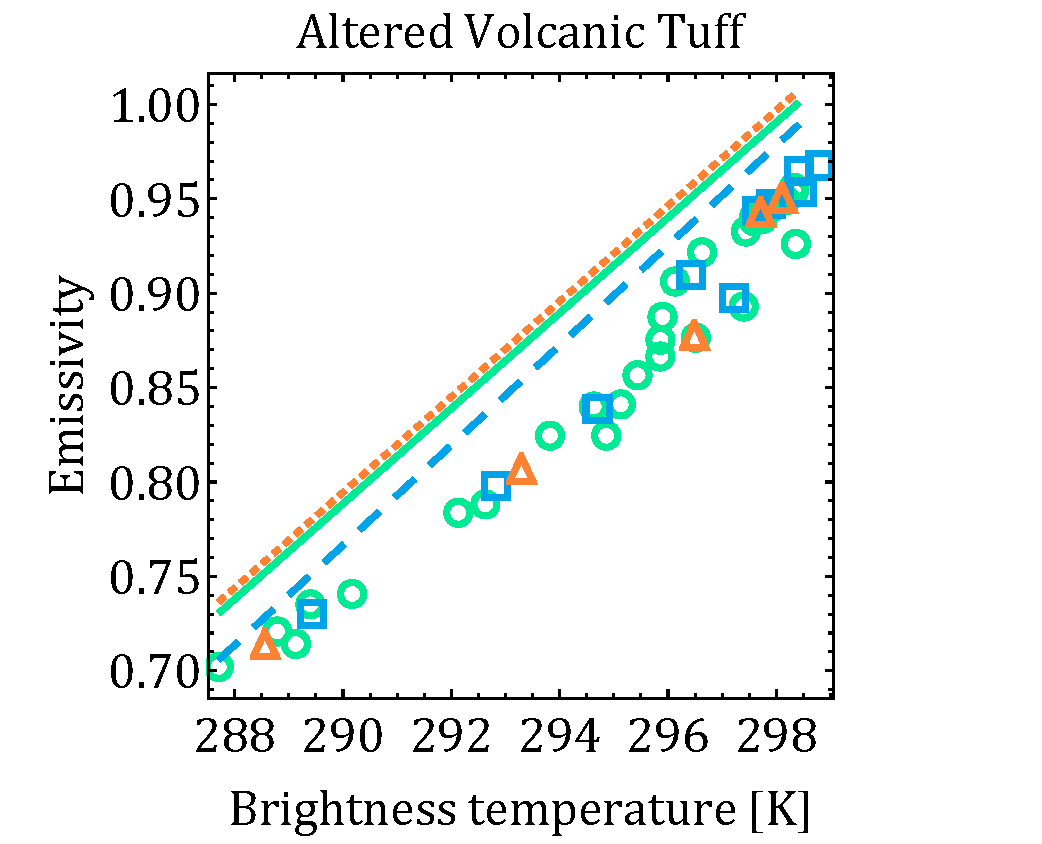
\includegraphics[width=7in]{pics/Chapter_03/pivov7}
\caption{Emissivity of Caspian Sea in different seasons obtained from ASTER standard product AST\_05, OSTES retrieval, and emissivity recomputation according to the temperature from AST\_08 and land-leaving and downwelling radiance from AST\_09T. Emissivities were extracted from area of size $40 \times 40$ pixels over pure and cloudless waterbody. Error bars display standard deviation.}
\label{fig:CaspianSeaEmissivity}
\end{figure*}

\section{Comparison with ASTER standard products}

The performance of the OSTES algortihm was also tested and compared with standard ASTER products. Testing is focused on: 1) investigating the impact of seasonal changes on emissivity retrievals, and 2) emissivity smoothness over homogeneous areas. Both tasks were performed on ASTER scenes containing large water bodies. For the first task we chose five scenes of the Caspian Sea acquired in various seasons of the year. For the second task we chose Lake Baikal. The list of all scenes used, together with their acquisition and processing date is given in Table \ref{table:ASTERScenes}. For every scene we downloaded ASTER standard products AST\_09T, AST\_08 and AST\_05 delivering land-leaving and downwelling radianace, surface kinetic temperature and surface emissivity, respectively. Product AST\_09T was used as input to the OSTES algorithm. The resulting temperature and emissivity was then compared with the AST\_08 and AST\_05 standard products. The emissivity variability over large and homogeneous area was chosen to be the quality indicator, since we are interested in the retrieval of material properties, which should be constant within the time and space.

\begin{table}[!t]
\renewcommand{\arraystretch}{1.5}
\caption{ASTER scenes used for algorithm testing}
\label{table:ASTERScenes}
\centering
\begin{tabular}{ccc}
\hline
Location & Acq date & Processing date \\ \hline
% &  &  \\
Caspian Sea & 11.02.2001 - 07:35:55 (UTC) & 19.11.2015 \\
Caspian Sea & 30.09.2001 - 07:35:57 (UTC) & 19.11.2015 \\
Caspian Sea & 29.06.2002 - 07:31:47 (UTC) & 19.11.2015 \\
Caspian Sea & 21.08.2004 - 07:29:35 (UTC) & 19.11.2015 \\
Caspian Sea & 13.11.2008 - 07:24:21 (UTC) & 19.11.2015 \\
Lake Baikal & 22.07.2002 - 04:17:29 (UTC) & 27.08.2015 \\
\hline
\end{tabular}
\end{table}

From the Caspian Sea scenes we chose samples of size $40 \times 40$ pixels over uniform, cloudless waterbody. These subsets were processed by the OSTES algorithm and the emissivity results were averaged for every scene. The results are plotted in Fig. \ref{fig:CaspianSeaEmissivity} along with the emissivities that were delivered in the AST\_05 product and averaged over the same spatial subset. In most cases the AST\_05 emissivity spectra appear to be closer to the sea water emissivity spectra taken from ASTER spectral library \cite{baldridge_aster_2009}. However, the temperature retrievals of extracted samples obtained by OSTES and TES are very close (not shown). The average temperature difference of AST\_08 and OSTES results computed from all Caspian Sea samples is 0.2\,K (s.d. 0.2\,K). The fact that the temperatures obtained with the two algorithms are very close, but the emissivities are not implies that the emissivity spectra from AST\_05 product are not consistent with temperature from AST\_08 product. We verified this inconsistency by taking the temperatures delivered in AST\_08 and the downwellig and land-leaving radiances delivered in AST\_09T and putting these into (\ref{eq:emissivityComputation}) to obtain emissivities that are different from what is in the AST\_05 product. These emissivity spectra derived from AST\_08 and AST\_09T, which we refer to as ``recomputed emissivities'', are depicted on Fig. \ref{fig:CaspianSeaEmissivity} as well. Comparing recomputed emissivity spectra and OSTES results shows that in scenes acquired on 29.6.2002 and 30.9.2001 are results similar. On the other hand OSTES results perform slightly better in scenes acquired on 11.2.2001, 21.8.2004 and 13.11.2008. Nevertheless, none of the emissivity spectra agrees with expected values.

The difference in emissivity obtained by the two versions of TES is further illustrated in the scene over Lake Baikal shown in Fig. \ref{fig:Bajkal}. In this figure the white squares on the images define a water body sample of size $90 \times 90$ pixels that was used to produce the values in the histograms below the images. The expected values of sea water emissivity (red vertical line) are included in the Fig. \ref{fig:Bajkal}. The histograms show the OSTES emissivity retrievals compared against the AST\_05 standard product, as well as the emissivity recomputed with respect to the temperature delivered by AST\_08 and land-leaving and downwelling radiance delivered by AST\_09T, as described in the previous paragraph. Inspection of the ASTER standard product AST\_05 shows step discontinuities in bands 10, 11 and 12 over the study sample, which is reflected in the bimodal distributions in the histograms and the noisy patterns in the left image. On the contrary, OSTES emissivity results are smoother and the histograms do not show any significant discontinuities. The recomputed and OSTES emissivity retrievals are similar. However, the OSTES emissivities tend to be closer to the expected values. In addition to the noise, striping is also visible in the image. This not consequence of the TES algorithm and is more deeply discussed in \cite{gillespie_residual_2011}. Even though the AST\_05 and OSTES emissivities differ significantly in some bands, the temperature retrievals are very similar. The average difference is 0.25 K (s.d. 0.18 K). Similar to the discussion regarding Caspian Sea emissivity retrievals, it can also be concluded in this case that none of the emissivity spectra have satisfying values.

\begin{figure*}[!t]
\centering
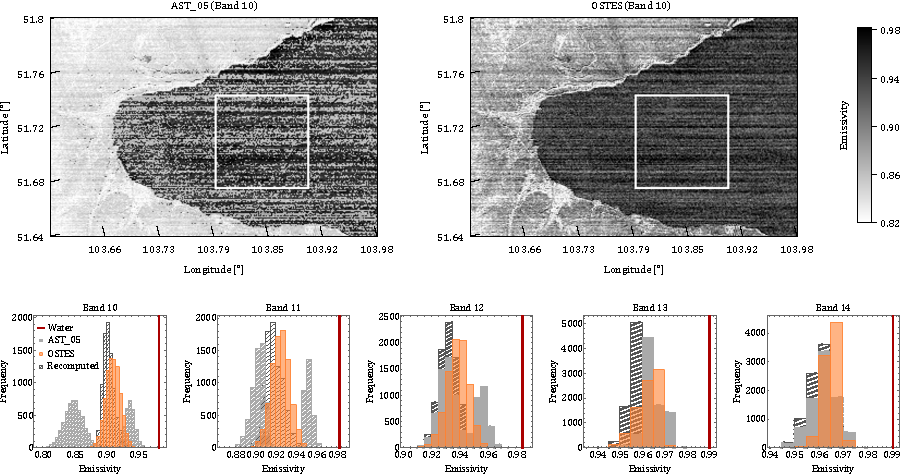
\includegraphics[width=7in]{pics/Chapter_03/pivov8}
\caption{
ASTER band 10 emissivity images of Lake Baikal obtained from ASTER standard product AST\_05 (upper left) and OSTES emissivity retrieval (upper right). In both images the same contrast stretching is used. The white square represents the area from which emissivity histrograms were created (lower panel). Histograms show distributions of AST\_05 emissivity, OSTES emissivity and recomputed emissivity according to the temperature from AST\_08 and land-leaving and downwelling radiance from AST\_09T. Line depicted in histograms indicates the expected value of water emissivity retrieved from ASTER spectral library \cite{baldridge_aster_2009}.}
\label{fig:Bajkal}
\end{figure*}

The discrapancies in shape and magnitude of emissivity spectra can be caused by various source of errors but the main error source has been attributed to imperfect atmospheric corrections. The impact of this error is evident mainly in cases of low spectral constast. Notable works discussing emissivity retrievals with low spectral contrast are \cite{tonooka_verification_2001, tonooka_validation_2005, tonooka_vicarious_2005, coll_temperature_2007, sobrino_accuracy_2007}. One suggested improvement is the water vapour scaling method \cite{tonooka_accurate_2005, gillespie_residual_2011}.

The step discontinuities in emissivity values over homogeneous area can occur due to various thresholds deciding how to treat the sample during processing. The original TES algorithm starts in the NEM module assuming a maximum emissivity spectra $\varepsilon_\mathrm{max}=0.99$. The NEM module is then restarted with refined $\varepsilon_\mathrm{max}$ according to the emissivity retrieved from the first NEM pass. Also,	 temperature and emissivity from NEM are reported as the result of TES algorithm if the correction for downwelling radiance is not possible. The original version of TES processes samples according to the MMD of emissivity spectra obtained from NEM module either by incorporating (\ref{eq:MMD}) or by presetting emissivity to $\varepsilon = 0.983$. Some authors \cite{gustafson_revisions_2006}, \cite{sabol_field_2009} have suggested that the value of the threshold used for classifying observations into groups with either low or high spectral contrast should be changed or completely removed. Observations with wrongly determined spectral contrast or observations with spectral contrast close to any threshold result in step discontinuities. On the contrary, the OSTES does not set any thresholds for materials with low spectral contrast and so it is expected to generate smoother results on homogeneous areas with low spectral contrast.

\section{Application to TASI Data}
